\documentclass[a4paper,oneside,10pt]{book}

%These tell TeX which packages to use.
\usepackage[utf8]{inputenc}
\usepackage[english,russian]{babel}
\usepackage{array,epsfig}
\usepackage{amsmath}
\usepackage{amsfonts}
\usepackage{amssymb}
\usepackage{amsxtra}
\usepackage{amsthm}
\usepackage{mathrsfs}
\usepackage{color}

\usepackage{caption,multicol}
\setlength{\columnsep}{0.2cm}
\usepackage{pdfpages}


%Here I define some theorem styles and shortcut commands for symbols I use often
\theoremstyle{definition}
\newtheorem{defn}{Definition}
\newtheorem{thm}{Theorem}
\newtheorem{cor}{Corollary}
\newtheorem*{rmk}{Remark}
\newtheorem{lem}{Lemma}
\newtheorem*{joke}{Joke}
\newtheorem{ex}{Example}
\newtheorem*{soln}{Solution}
\newtheorem{prop}{Proposition}


%Pagination stuff.
\setlength{\topmargin}{-.3 in}
\setlength{\oddsidemargin}{0in}
\setlength{\evensidemargin}{0in}
\setlength{\textheight}{9.in}
\setlength{\textwidth}{6.5in}
\pagestyle{empty}



\begin{document}


\begin{center}
	{\large  ТАУ \hspace{0.1cm} Лабораторная работа \textnumero 5}

	\vspace{5pt}
	\textit{\large Регуляторы САУ}\\ %You should put your name here
	\vspace{10pt}
	Due: 22 мая %You should write the date here.
\end{center}

\vspace{0.2 cm}



Пусть объект управления с одним входом~$ x(t) $ и одним выходом~$ y(t) $ задан передаточной функцией~$ P(s) $:

\begin{equation*}
	P(s) =
	\dfrac{a_0}
	{b_3 s^3 + b_2 s^2 + b_1 s +1} ,
\end{equation*}

где коэффициенты  определяются согласно варианту $ n $:
\begin{equation*}
	a_0 = n, \quad b_1 = n,
\end{equation*}

а значения $b_2$, $b_3$ выбираются из области устойчивости системы.

САУ с обратной связью определена следующим образом:

\begin{figure}[h]
	\centering
	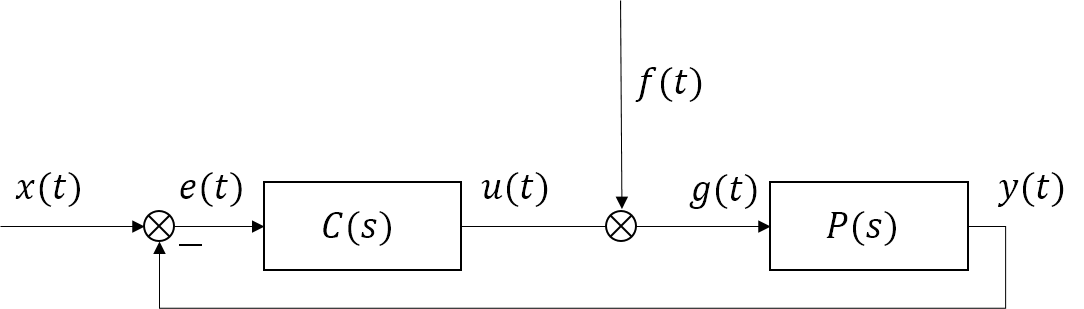
\includegraphics[width=0.8\linewidth]{tau.png}
	\caption{Схема САУ}
\end{figure}
здесь $C(s)$~--- регулятор,
$e(t)$~--- ошибка управления,
$f(t)$~--- возмущающее воздействие,
$u(t)$~--- управляющее воздействие.

\subsection*{\textit{Задания}}
С использованием пакета \textit{control}:
\begin{enumerate}
	\item
	      Построить реакцию на нулевой сигнал, гармонический сигнал $sin(\omega t)$ и некоторое возмущающее воздействие~$f(t)$.
	\item
	      Пострить регуляторы~$C(s)$:
	      \begin{itemize}
		      \item
		            пропорциональный,
		      \item
		            интегральный,
		      \item
		            дифференциальный (2),
		      \item
		            ПИ,
		      \item
		            ПД,
		      \item
		            ПИД.
	      \end{itemize}

	      Определить вид передаточных функций:
	      $W_{y,x}$, $W_{y,f}$,
	      $W_{u,x}$, $W_{u,f}$,
	      $W_{e,x}$, $W_{e,f}$.


	      Рассмотреть регуляторы с различными коэффициентами. Подобрать значения коэффициентов так, чтобы гарантировать устойчивость при некоторой точности управления (если это возможно).

	      Для каждого устойчивого регулятора~$C(s)$ провести эксперименты и построить:
	      \begin{itemize}
		      \item
		            $y_x(t) =  W_{y,x}(p)x(t)$,
		      \item
		            $y_f(t) =  W_{y,f}(p)f(t)$,
		      \item
		            $y(t)$,
		      \item
		            $u_x(t) =  W_{u,x}(p)x(t)$,
		      \item
		            $u_f(t) = W_{u,f}(p)f(t)$,
		      \item
		            $u(t)$,
		      \item
		            $e_x(t) =  W_{e,x}(p)x(t)$,
		      \item
		            $e_f(t) = W_{e,f}(p)f(t)$,
		      \item
		            $e(t)$.
	      \end{itemize}

	      Пронализировать полученные результаты, сделать выводы.
\end{enumerate}



\end{document}


